\newcommand{\splitrule}[2]{
	\parbox[t]{4.25in}{
		\parbox{2.75in}{#1}\parbox{1.25in}{#2}}}

\newcommand{\gensplit}[2]{
	\parbox[t]{4in}{
		\parbox{2in}{#1}\parbox{2in}{#2}}}

\newcommand{\gentrisplit}[3]{
	\parbox[t]{4.5in}{
		\parbox{1.5in}{#1}\parbox{1.5in}{#2}\parbox{1.5in}{#3}}}

\chapter{Exhibit of a Working Model of a Perception-Dissociator}

\section*{\textsc{Statement of Objectives}}

To construct a model of a machine a thousand years before the machine 
itself is technologically feasible---to model a technological breakthrough a 
thousand years before it occurs 

\begin{sysrules}
(Analogies: constructing a model of an atomic power plant in ancient 
Rome; chess-playing-machine hoaxes of 19th-century Europe as 
models of computers; Soviet Cosmos Hall at Expo 67 as model 
of anti-gravity machine) 

To construct the model almost entirely from the visitors coming to see it, so 
that each visitor regards the others as the model! 

What the hypothetical perception-dissociator will do that is not 
possible now: 
\end{sysrules}

\begin{itemize}
\item Physically alter the world (relative to you): sound disappears; sights and 
touches are dissociated; other people unconsciously signal you. 

\item Physically, "psychoelectronically" induce conditioned reflexes in your 
nervous system. Physically break ddwn your sense of time. 
\end{itemize}

{ \centering
	\large
	[\textsc{Invitation}] \par}

{ \centering 
Because of your interest in technology and science, you are invited to visit \\
	\textsc{Exhibit of a Working Model of a} \\
	\textsc{Perception-Dissociator} \\
Sponsored by (legitimate sponsor) Open continuously from (date) \\
to (date) At (lunar colony or space station) \par
	}

"The perception-dissociator is a machine which is the product of a 
technology far superior to that of humans. With it, a conscious organism can 
drastically transform its psychophysical relation to objects and to other 
conscious organisms\ldots The exhibit spotlights the technical interest of the 
perception-dissociator, giving the visitor a working model of the machine 
which he can use to 'transform' himself." ---from the Guidebook 

It isn't possible for this exhibit to be open or public, because of the nature of 
the model. You have been invited in the belief that you will be a cooperative 
visitor. Come alone. Don't discuss the exhibit at all before you see it; and 
don't discuss it afterwards except with other ex-visitors. Come prepared to 
spend several hours without a break. There will be absolutely no risk or 
danger to you if you follow instructions. 

\section*{\textsc{To the Director}}

Exhibit requires two adjacent rooms, on moon or other low-gravity 
location, so that humans can easily jump over each other and fall without 
being hurt. First room, the anteroom, has "normal" entrance door leading in 
from "normal" human world. Is filled with chairs or school desks. At far 
corner from normal door is two-step lock, built in anteroom, connecting 
rooms. Normai door on hinges leads from anteroom into first step of lock. 
Sliding panel door leads into second step; and smooth curtain with slit in 
middle leads into the exhibit hali. Another sliding door leads from lock's 
first step directly back out to normal human world, bypassing anteroom. 
Shelf required in first lock to check watches and shoes. 

Exhibit hall large and empty with very high ceiling (Fuller dome?). I 
Room must be strongly lighted, so that objects in front of closed eyes will 
cast highly visible shadows on eyelids. Room's inner surfaces must be 
sound-absorbing, and moderate noise must be played into room to mask 
accidental sounds; thus humans will cease to notice sound. Floor must be of 
hard rubber or other material that will not splinter, and will not be too hard 
to fall and crawl on. 

Exhibit open continuously for days. Invite people who will seriously 
try to play along---preferably engineers; and invite many of them, because 
is better to have many in exhibit. Sample invitation enclosed. Attendants 
working in shifts must be at two posts throughout. Try to keep surprising 
features of exhibit secret from those who have not been through it. 

Procedure. Visitor arrives and enters anteroom. Entrance attendant 
gives him a Guidebook and sends him to sit down and start reading. Then 
visitor goes to lock. Lock attendant must try hard to see that no more than 
one visitor is in lock at a time. If lock is empty of visitors, attendant lets 
entering visitor into first step, checks his watch and shoes, and sends him 
alone into second step and on to exhibit room. When visitor comes out of 
exhibit hall for any reason, he must be gotten into first step, and then 
attendant sends him out the exit. When a visitor comes out, he just goes out 
and doesn't go back in. 

{\centering
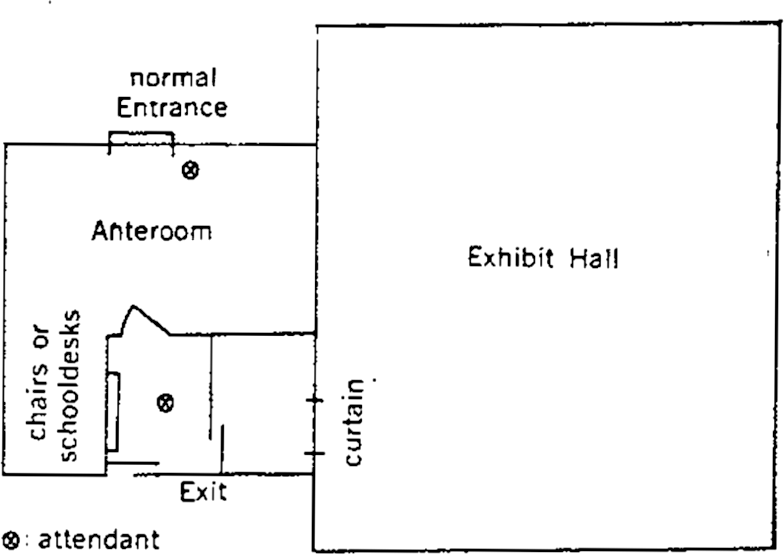
\includegraphics[scale=1]{img/dissociatordiag}\par
}

\clearpage
\newcommand\intab[1]{
\framebox[1.1\width]{\parbox[c][2.5em]{4em}{
	\centering\Huge #1}}}

\newcommand\righttab[1]{{\raggedleft\intab{#1}\par}}

\newcommand\lefttab[1]{{\raggedright\intab{#1}\par}}

{\righttab{1}

\centering

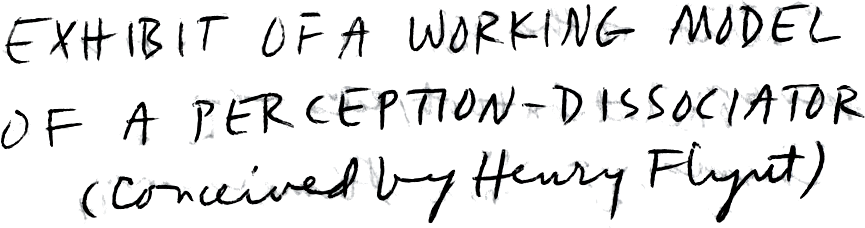
\includegraphics[width=4in]{img/guidebook_01}

\vfill


\includegraphics[width=3.5in]{img/guidebook}

\vfill

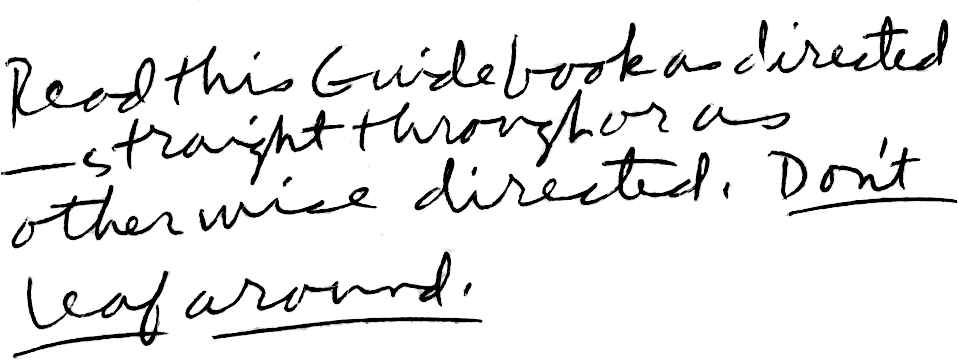
\includegraphics[width=4in]{img/guidebook_02}

\vfill

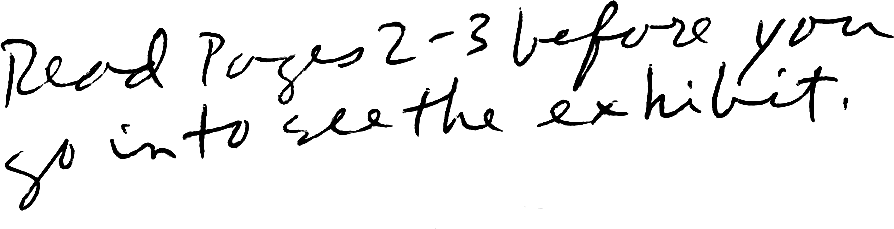
\includegraphics[width=4in]{img/guidebook_03}

\vfill\clearpage}

\lefttab{2}

\uline{Introduction.} The perception-dissociator is a machine which is the 
product of a technology far superior to that of humans. With it, a conscious 
organism can drastically transform its psychophysical relation to objects and 
to other conscious organisms. When the organism has transformed itself, 
sound disappears, time is immeasurable; and the relation between seeing and 
touching becomes a random one. That is, the organism never knows whether 
it will be able to touch or feel what it sees, and never knows whether it will 
be able to see what it touches or what touches it. The world ceases to be a 
collection of objects (relative to the physically altered organism). Further, 
the machine induces a pattern of communication in the organism's nervous 
system, an \uline{involuntary} pattern of responses to certain events, to help the 
organism cope with the invisible tactile phenomena. A dimension is added of 
involuntarily relating to other organisms as unconscious signalling devices. 
The transformation induced by the machine is permanent unless the 
organism subsequently uses the machine to undo it. 


The perception-dissociator is not conscious or alive in any human sense. 
The components of the machine that the user is aware of are: 
\begin{enumerate}
	\item Optical phenomena that are seen---\enquote{sights.} 
	\item Solid or \uline{massive} phenomena that are felt cutaneously---\enquote{touches.} 
\end{enumerate}
If the user tries to touch a sight, he may not be 
able to feel anything there. If he looks for a component that touches him, he 
may not be able to see it. 

\vfill

(Keep reading) 

\vfill

\clearpage

\righttab{3}

In other words, from the beginning the machine has properties that the 
entire world comes to have to the transformed organism. 

The exhibit spotlights the technical interest of the 
perception-dissociator, giving the visitor a working model of the machine 
which he can use to \enquote{transform} himself. Nothing is said about the purpose 
of the perception-dissociator in the society that can make one. The model is 
sophisticated enough that it can run independently of the visitor's will, and 
can affect him. In fact, the visitor may be hurt if he doesn't follow the 
instructions for using the machine. 


When you have absorbed the above, go to the entrance and be admitted 
to the exhibit. You must check your shoes, and your watch (if you have 
one), with the attendant. As you enter, turn this page and begin reading Page 
4. 

\clearpage

\lefttab{4}
\vfill 
\textsc{Do not talk or make any other uncalled-for noise.}

\vfill 

Be prepared for the touch of pulling your feet out from under you 
from behind. Don't resist; just fall forward, break your fali with your arms 
(and retrieve this Guidebook). The floor is not hard and the gravity is weak, 
so the fall should leave you absolutely unhurt. 

\plainbreak{2}

\textsc{Avoid all touches (except floor and yourself) unless directed otherwise.}


\plainbreak{2}

(You have been directed not to resist having your 
feet pulled out from under you.) 
\plainbreak{2}

\textsc{In effect, if you bump into a solid object or step on one, draw back. Remember
that you avoid touches by your tactile senses alone.}
Whether your eyes are open or closed makes no difference. It is not necessary to avoid 
sights unless you touch something. 

\plainbreak{2}

There may be the touch of being pushed forward at your shoulder 
blades. Don't resist; just move forward. 

\plainbreak{2}

As for the sights in this model, it happens that they will be humanoid. 
All the human appearances other than you in the exhibit hall are sights from 
the machine. This is just the way the model is; don't give it a thought. Sights 
may appear or disappear (for example, at the curtain) while you are looking. 

\plainbreak{2}

I am referring to the components of the model with the names of the 
components of the perception-dissociator. 

\plainbreak{2}

As soon as you understand the above and are prepared to remember 
and follow the instructions, go immediately to Page 6. 

\vfill 

\clearpage

\righttab{5}

  \vfill
\gentrisplitmath{
  \bigprobly{\jumpsover{
      \scoot{s_1}}{
      \probly{\shadows{s_2}{\eyeO{u}}}}}}{
  \jumpsover{s}{
    \jumpsover{t}{
      u}}}{
  \tackles{
    \crawl{\eyeC{u}}}{t}}
	
  \vfill
\gentrisplitmath{
  \begin{gathered}
    \shadows{s}{}\\
    \blows{t}{}
  \end{gathered}
  \:\:\:\eyeC{u}}
  {\shadows{\crouch{u}}{s_2}}
  {\jumpsover{\scoot{u}}{
    \pushes{
      \belowU{\eyeC{s_1}}}{
      \belowU{\eyeO{s_2}}}}}

  \vfill
\gentrisplitmath{
  \tackles{
    \eyeC{\crawl{u}}}{
    \eyeC{\aboveU{t}}}}
  {\probly{
    \stepson{s_1}
            {\eyeC{\crawl{s_2}}}}}
  {\crawl{t}
  \:\dfrac{\pushes{\vee}{}}{\blows{\wedge}{}}\:u}

  \vfill

\gensplitmath{\flee{\scoot{\eyeC{u}}}}
{\begin{array}{c}\begin{array}{c c}
    \pushes{s_1}{s_2}&\pushes{s_3}{s_1}\\\hline
    &\pushes{s_1}{s_2}\end{array}
  \left(\begin{array}{c}\tackles{s_1}{s_3}\\
    \jumpsover{s_2}{u}\end{array}\right)\\\:\:
  {\renewcommand{\arraystretch}{0.5}
    \begin{array}{l@{}p{8em}}
      \pushes{s_2}{s_3}\,&\hrulefill\\
      \hrulefill&\,\pushes{s_2}{s_3}\\
      \pushes{s_3}{s_1}\,&\\\end{array}}\end{array}}

\vfill

\gentrisplitmath{
	\left(
	  \begin{gathered}
            \dfrac{\tackles{\eyeC{s_1}}{s_2}}
		  {\tackles{\eyeC{s_1}}{s_2}}\\
	    \dfrac{\pushes{s_2}{s_3}}
		  {\pushes{s_2}{s_3}}
	  \end{gathered}
	\right)}
{\jumpsover{\left.\begin{gathered}
	s\\
	t
\end{gathered}\right.}{u}}{
\dfrac{\dfrac{\dfrac{\eyeC{\crawl{s_1}}}
                    {\aboveU{\eyeO{s_1}}} \: \shadows{u}{s_1}}
	     {\eyeO{\scoot{s_1}}} \: \probly{\pushes{s_1}{s_2}}}
      {\eyeO{\belowU{s}}} \: \eyeC{u}}

\vfill

\gentrisplitmath{\jumpsover{u}{\belowU{s_3}}}
  {\left(\;\begin{array}{c}
	  \jumpsover{\scoot{s_1}}{\eyeO{u} }\\
  \shadows{s_2}{u}
  \end{array}\;\right)}
  {\eyeO{s_3}}

\vfill
\gensplitmath{\jumpsover{u}{\begin{array}{c}
	\pushes{\eyeC{\belowU{s_1}}}{\eyeC{\belowU{a_1}}}\\
	\pushes{\eyeC{\belowU{s_2}}}{\eyeC{\belowU{s_1}}}
\end{array}}}{\jumpsover{\crouch{u}}{\probly{\shadows{s_1}{\eyeO{s_2}}}}}

\vfill
\gentrisplitmath{\jumpsover{t_1}{\pushes{t_2}{\scoot{u}}}}
{\shadows{s}{\shadows{u}{s}}}
{\left(\begin{array}{c}
	\jumpsover{s_2}{u} \\ \hline
	\tackles{s_1}{s_3} \\
\jumpsover{s_2}{u}\end{array}\right)
\begin{array}{c}
	\jumpsover{u}{s_1} \\ \hline
	\jumpsover{u}{s_3} \\
	\\
	\\
\end{array}}
\clearpage

% \img{dissoceqns}

\clearpage
\lefttab{6}
\section{First Phase}
You will now begin the first phase of perception-dissociation by the 
machine. Throughout this phase, you walk erect. 

Instructions for operating the machine and for protecting yourself from 
it will be given both in English and in an abbreviated symbolism. It is 
important to master the symbolism, because later instructions can't be 
expressed without it. 

\begin{itemize}
\item u means you 

\item $s$, $s_1$, $s_2$, $s_3$ mean different sights from the machine 

\item $t$, $t_1$, $t_2$, $t_3$ mean different touches from the machine 

\item $\eyeO{a}$ means $a$'s eyes are open or $a$ opens its eyes 

\item $\eyeC{a}$ means $a$'s eyes are shut or $a$ shuts its eyes 

\item $\blows{a}{b}$ means $a$ blows on $b$'s hand 

\item $\pushes{a}{b}$ means $a$ pushes $b$, typically from behind 
($a$ holds Guidebook under arm or elsewhere) 

\item $\jumpsover{a}{b}$ means $a$ jumps over $b$, crossing completely above $b$ (weak gravity should make this easy) 

\item $\shadows{a}{b}$ means $a$ rapidly waves both hands in front of and near $b$'s eyes so that 
	moving shadows are cast on $b$'s eyes ($a$ \enquote{\term{shadows}} $b$) 

\item $\tackles{a}{b}$ means $a$ pulls $b$'s ankles back and up and immediately lets them go, so 
	that $b$ falls forward ($a$ \enquote{\term{tackles}} $b$) 

\item $\stepson{a}{b}$ means $a$ jumps and falls on $b$, or $a$ steps on $b$ 

\item $\flee{a}$ means $a$ rapidly moves aside 

\item $\probly{}$ parentheses around the symbol for an action mean the action will 
probably happen 

\item A line of action symbols constitutes an instruction. The order of symbols 
indicates the order of events. If one symbol is right above another, the 
actions are simultaneous. 
\end{itemize}

\vfill
\textsc{You may always turn back to these explanations if you forget them.}

\vfill
(Keep reading) 

\vfill
\clearpage
\righttab{7}

Instructions 1--3 apply \textsc{when your eyes are open.}

\vskip 0.75em

\newcommand{\eqnAB}{
	\begin{equation*}
	\left.\begin{gathered}
		\eyeO{s_1}\\
		\eyeO{u}
	\end{gathered}\right.\:\left.
		\begin{gathered}
			\eyeC{s_1}\\
			\probly{\stepson{t}{u}}
		\end{gathered}\right.\:
	\flee{u}
	\end{equation*}}

\begin{enumerate}[label=\arabic*.,nosep, wide]
	\item \splitrule{If you see a sight close its eyes, a heavy touch from the machine may be falling toward you.
		You must instantly jump aside.}{\eqnAB}

		\vskip 0.5em

\textsc{You must follow this and succeeding instructions as long as you stay in the exhibit. Stay with each instruction until you have it thoroughly in memory; and check out the symbolic version so you learn to read the symbols.}
		\vskip 0.75em

\item \splitrule{If a sight in front of you jumps over you, a touch may be about to tackle you. You must instantly jump to one side. }{
\begin{equation*}
	\eyeO{u}\:\left.\begin{gathered}
		\jumpsover{s}{u} \\
		\probly{\tackles{t}{u}}
	\end{gathered}\:\right.\flee{u}
\end{equation*}
	}

\vskip 0.75em

\item \splitrule{If a sight waves its hands in front of your open eyes, a touch may be about to shove from behind.
	Jump to one side. }{\begin{equation*}
  \eyeO{u}\:\left.\begin{gathered}
    \shadows{s}{u}\\
    \probly{\pushes{t}{u}}
  \end{gathered}\:%
  \right.\flee{u}
\end{equation*}}


\vskip 0.75em

\textsc{If there are any sights, try standing around and following these instructions for a short while.}

\vskip 0.75em

\item \splitrule{If you close your eyes, you must keep them closed until a touch tackles you, a touch shoves you, or you can't keep your mind on the exhibit (which you should also consider to be an effect of the machine). Then you immediately open your eyes.}{\begin{equation*}
    \quad\eyeC{u}\:%
      \dfrac{\tackles{t}{u}}{
        \dfrac{\pushes{t}{u}}{
          u\:\text{inattentive}}}%
  \:\eyeO{u}
\end{equation*}}

\vskip 0.75em

\emph{(A horizontal line between action symbols means \emph{or.} With it, instructions can be combined)}

\vskip 0.75em

\textsc{The next three instructions tell you what to do when your eyes are closed. Learn them well.}

\vskip 0.75em

\item \splitrule{If you feel a breath blowing on one of your hands, a touch may be falling on you. You must instantly jump to the side away from the breath.}{\begin{equation*}
  \eyeC{u}\:\begin{gathered}
    \blows{t_1}{u}\\
    \probly{\stepson{t_2}{u}}
  \end{gathered}
  \flee{u}
\end{equation*}}

\vfill

\textit{(Turn page and continue) }

\vfill

\clearpage

\lefttab{8}

\vfill
\item If your closed eyes are shadowed, a touch may be about to tackle 
you. You must instantly jump aside. 
\begin{equation*}
  \eyeC{u}\begin{gathered}
    \shadows{s}{u}\\
    \probly{\tackles{t}{u}}
  \end{gathered}
  \:\:\flee{u}
\end{equation*}

\vfill
\item If you sense a massive touch going above your head, another touch 
may be about to shove you from behind. Jump aside. 

  \[\eyeC{u}\:\begin{gathered}
    \jumpsover{t_1}{u}\\
    \probly{\pushes{t_2}{u}}
  \end{gathered}
  \:\:\flee{u}\]

\vfill
\item If you have any time left over from following other instructions, 
close your eyes and go around with your hands in front of you, shoving 
touches whenever you feel them. 

\[\eyeC{u} \:\:\: \pushes{u}{t}\]

\vfill

\textsc{Now try instr. 8, remembering and following the other instructions about closed eyes (instr. 4--7).
When you have to open your eyes again, as per instr. 4, check anything you forgot: and then go to the
succeeding instructions. Now---close your eyes.}

\vfill

\textsc{The next three instructions apply when your eyes are open.}

\vfill
\item If you see a sight falling toward or about to step on another sight 
whose eyes are open, run until you face the sight on the ground and close 
your eyes. 

\textsc{Before you follow this instruction you must have mastered the preceeding instructions about closed eyes.}

\[\eyeO{u}\:\eyeO{s_2}\:\probly{\stepson{s_1}{s_2}}\:\eyeC{u}\]

\vfill
\textit{(Keep going) }

\clearpage

\righttab{9}

\vfill
\item If you see a sight about to tackle another whose eyes are \uline{open}, run 
until you face the sight about to be tackled and jump over both sights. If the 
sight about to be tackled has \uline{closed eyes}, you must immediately shadow 
them. 

\vfill
  \[\eyeO{u}\dfrac{%
      \eyeO{s_2}\quad\probly{\tackles{s_1}{s_2}}\quad\jumpsover{u}{s_1 s_2}%
    }{%
      \eyeC{s_2}\quad\probly{\tackles{s_1}{s_2}}\quad\shadows{u}{s_2}%
    }\]

\vfill
\item If you see a sight about to push another with open eyes from 
behind, you must shadow the sight about to be pushed. But if the sight 
about to be pushed has closed eyes, you must immediately jump over both 
sights. 


\vfill

  \[\eyeO{u}\dfrac{%
    \eyeO{s_2}\quad\probly{\pushes{s_1}{s_2}}\quad\shadows{u}{s_2}
    }{%
      \eyeC{s_2}\quad\probly{\pushes{s_1}{s_2}}\quad\jumpsover{u}{s_1 s_2}
    }\]

\end{enumerate}

\vfill
You must now put all the instructions into practice until you have 
learned them thoroughly by doing as they say. In other words, carry out 
Instr. 8, and the other instructions as they apply. 

\vfill
If you can't practice the instructions because you still have not seen a 
sight or felt a touch, skip directly to Page 18. 

\vfill

Learning the instructions in practice should take a good while. When 
you have mastered them, the first phase is over. Turn to Page 10 and \textit{begin the second phase}.

\vfill

\clearpage

\lefttab{10}

\section{Second Phase}

\vfill
You are now in the second phase of transforming yourself with the 
perception-dissociator. Throughout this phase, you must stoop or crouch 
somewhat. That is, you must keep yourself below the height of your neck 
when you stand straight---except when you jump over a sight. The symbol is 
$\crouch{u}$. $\eyeC{\crouch{u}}$ means that you crouch and close your eyes. \emph{Now crouch.}

The numbered instructions for this phase are so similar to those in the 
preceeding phase that they will be given in symbols only. Changes are noted 
parenthetically. You may turn back if you forget symbols. 

\vfill
\begin{enumerate}
	\gensplit{\item\BEQ{
	\left.\begin{gathered}
	\eyeO{s_1}\\
	\eyeO{\crouch{u}}
	\end{gathered}\right.
	\:\:
		\left.\BG{
		\eyeC{s_1}\\
		\probly{\stepson{t}{u}}
	}\right.
	\:\:
		\flee{u}}}
{\item\BEQ{
	\eyeC{\crouch{u}}\:
		\BG{\jumpsover{s}{u}\\
		\probly{\tackles{t}{u}}}\:
		\flee{u}}}

\vfill
\gensplit
  {\item\BEQ{\eyeC{\crouch{u}}\:
	     \BG{\blows{t}{u}\\
		 \pushes{t_2}{u}}\:
             \flee{u}}}
 {\emph{(change: component blows on you instead of shadowing you)}}

\vfill
\gensplit{\item\BEQ{
  \eyeC{\crouch{u}}\:\:
  \dfrac{\tackles{t}{u}}
	{\dfrac{\pushes{t}{u}}
	       {u\:\text{inattentive}}}\:\:
  \flee{u}}}
  {\item\BEQ{
  \eyeC{\crouch{u}}\:\:
  \BG{\blows{t_1}{u}\\
      \probly{\tackles{t_2}{u}}}\:\:
  \flee{u}}}


\vfill
\gensplit{\item\BEQ{
  \eyeC{\crouch{u}}\:\:
  \BG{\shadows{s}{u}\\
      \probly{\tackles{t}{u}}}\:\:
  \flee{u}}}
  {\item\BEQ{
  \eyeC{\crouch{u}}\:\:
  \BG{\jumpsover{t_1}{u}\\
      \probly{\pushes{t_2}{u}}}\:\:
  \flee{u}}}

\vfill
\gensplit{\item\BEQ{
  \eyeC{\crouch{u}}\qquad\pushes{u}{t}}}
{The big change comes next. 
\plainbreak{2}
\emph{(Keep going)}}

\vfill

\clearpage
\righttab{11}

\vfill
\item \BEQ{\begin{array}{c c c c r}
		\eyeO{\crouch{u}} &
		  \eyeO{s_2} &
		  \probly{\stepson{s_1}{s_2}}& 
		  \eyeC{u} & \text{\uline{and also}} \\
		\eyeO{\crouch{u}} &
		  \eyeC{s_2} &
		  \probly{\stepson{s_1}{s_2}} & 
		  \blows{u}{s_2} & \end{array}}

\vfill
That is, if you see a sight falling or stepping on another sight with \uline{closed eyes}, you must immediately blow on the sight on the ground. This is an addition.
\vfill
\item \[
  \eyeO{\crouch{u}}\:\:
  \begin{array}{c c c}
    \eyeO{s_1} & \probly{\tackles{s_1}{s_2}} &
      \jumpsover{u}{s_1 s_2} \\
    \hline
    \eyeC{s_1} & \probly{\tackles{s_1}{s_2}} &
      \shadows{u}{s_2} \\
  \end{array}
\]

\vfill
\splitshort{\item \[
  \eyeO{\crouch{u}}\:\:
  \begin{array}{c c c}
	  \eyeO{s_2} & \probly{\pushes{s_1}{s_2}} & \blows{u}{s_2} \\
	  \hline
	  \eyeC{s_2} & \probly{\pushes{s_1}{s_2}} & \jumpsover{u}{s_1 s_2} \\
  \end{array}\]}
  {\emph{(change: you blow on $s_2$)}}

\vfill
So far there have been only three changes in the instructions. Memorize 
them. Then go on to Instr. 12, which is new, and carry it out along with the 
other eleven instructions. 

\vfill
\textsc{As soon as you have put any changed instruction (3, 9, or 11) into practice,
the second phase is over. Turn to page 12 and the third phase.}

\vfill
If you can't practice the instructions because all the components have 
vanished, skip to Page 18. 

\vfill

\splitrule{\item Adding to Instruction 8, if you have time left over from following other instructions, you may also keep your eyes open and jump over, blow on, or shadow sights.}{\[
	\eyeO{\crouch{u}}\:\:
	\begin{array}{c}
		\jumpsover{u}{s} \\ \hline
		\shadows{u}{s} \\ \hline
		\blows{u}{s} \\
	\end{array}
\]}
\end{enumerate}

\clearpage 

\lefttab{12}

\section{Third Phase}

Throughout the third phase, you must squat or move on your hands 
and knees. That is, you must always keep yourself below the height of your 
waist when you stand straight---unless you are able to jump over a sight from 
your low position. The symbol is $\crouch{u}$. Now get down. 

Instr. 1--7 from the last phase apply here without change. They are thus 
stated in the most abbreviated form. 

\vfill

{1--3. \parbox[t]{1.75in}{\[
	\eyeO{\crouch{u}} \:\: 
	\begin{array}{c}
		\eyeC{s} \\
		\probly{\stepson{t}{u}} \\ \hline
		\jumpsover{s}{u} \\
		\probly{\tackles{t}{u}} \\ \hline
		\blows{t_1}{u} \\
		\probly{\pushes{t_2}{u}}
	\end{array}\:\:
	\flee{u}
\]\vskip 3.5em} 4--7. \parbox[t]{2.4in}{\[
	\eyeC{\crouch{u}}\:\:
	\dfrac{
		\:\:
	  \begin{array}{c}
	    \tackles{t}{u} \\ \hline
	    \pushes{t}{u} \\ \hline
	    u \:\:\text{inattentive} \\
	  \end{array}\qquad
	\eyeO{u}\:\:}
{\begin{array}{c}
	    \blows{t_1}{u} \\
	    \probly{\stepson{t_2}{u}} \\ \hline
	    \shadows{s}{u} \\
	    \probly{\tackles{t}{u}} \\ \hline
	    \jumpsover{t_1}{u} \\
	    \probly{\pushes{t_2}{u}} \\
	 \end{array}\qquad
	 \flee{u}}
 \]}

\vfill
The biggest change comes next. 

\vfill
8. If you have any time left over, close your eyes and go around with 
your hands in front of you. If you encounter touches standing higher than 
you, tackle them. If you encounter touches as near the ground as you, shove 
them. You must be sensitive and judge heights with eyes closed. 

\vfill

\[
	\eyeO{\scoot{u}}\:\:\begin{array}{c c}
		\aboveU{t} \tackles{u}{t} \\ \hline
		\belowU{t} \pushes{u}{t} \\
	\end{array} \:\:
	\left( \begin{gathered}
		\aboveU{t} \: \text{\textsc{means "if $t$ stands high relative to you"}} \\
		\belowU{t} \: \text{\textsc{means "if $t$ is near ground relative to you"}}
	\end{gathered} \right)
	\]

	\vfill

9. \parbox{1.5in}{No change.}\parbox{2in}{\[
	\eyeC{\scoot{u}} \:\: \begin{array}{c c c}
		\eyeC{s_2} & \probly{\stepson{s_1}{s_2}} & \eyeO{u} \\ \hline
		\eyeO{s_2} & \probly{\stepson{s_1}{s_2}} & \blows{u}{s_2}
	\end{array}
\]}
\vfill

\vfill
(Keep going) 

\clearpage
\righttab{13}

\vfill 

10. \gensplit{The previous Instr. 10 applies if $s_2$ is near the ground, that is, it applies unless $s_2$ is too high for you to jump or shadow it.}{\[
	\eyeC{\scoot{u}} \: \begin{array}{c c c}
		\belowU{\eyeC{s_2}} & \probly{\tackles{s_1}{s_2}} & \jumpsover{u}{s_1 s_2} \\ \hline
		\belowU{\eyeO{s_2}} & \probly{\tackles{s_1}{s_2}} & \shadows{u}{s_2}
	\end{array}
\]}

\vfill 

11. \gensplit{\[
	\eyeC{\scoot{u}} \:\: \eyeC{s_2} \:\: \probly{\pushes{s_1}{s_2}} \:\: \blows{u}{s_2}
\]}{The second half of the previous Instr. 11 is dropped. }

\vfill 
\vskip 1.5em
Except for the instruction to tackle touches, the changes are simply 
limitations to make the instructions feasible for $u\sfrac{1}{2}$. They should be easy 
to remember. 

\vskip 1.5em

You will next go on to Instr. 12, and carry it out along with the other 
instructions. As soon as you encounter an actual situation where you cannot 
act because $u\sfrac{1}{2}$, the third phase will be over. 
\textsc{At that point you must turn to page 14 and the fourth phase.}

\vskip 1.5em
If you can't carry out the instructions because all the components have 
vanished, the third phase is over. Turn to Page 14 and the fourth phase. 

\vskip 1.5em

\vfill 

12. \gensplit{Adding to Instr. 8, if you have time left over, you may also keep 
your eyes open and blow on sights. You may also shadow or jump over 
sights unless they are too high. }{ \vfill 
\[\eyeC{\scoot{u}} \:\: \dfrac{\blows{u}{s}}{
	\belowU{s} \:\: \dfrac{\blows{u}{s}}{\jumpsover{u}{s}}}
\]}
\vfill 
\clearpage
\lefttab{14}

\section{Fourth phase}



You are in the fourth phase of perception-dissociation. Throughout this 
phase, you must crawl on your stomach (keep below knee height). The 
symbol is $u\sfrac{1}{4}$. Now get on the floor. 

You can no longer be tackled, nor can you jump. Thus, the numbered 
instructions are greatly limited, and they will be restated fully. 

\vfill

\textsc{The first two instructions apply when your eyes are open.}

\vfill

\begin{enumerate}
\gensplit{\item If you see a sight close its eyes, a touch may be falling or stepping on you, and you must immediately scramble aside.}
{\[\begin{array}{c c}
	\eyeO{s_1} & \eyeC{s_1} \\
	\eyeO{\crawl{u}} & \probly{\stepson{t}{u}}
\end{array} \:\: \flee{u}\]}

\vfill

		{\centering \parbox{2in}{
\item \[ \eyeO{\crawl{u}} \:\: \begin{array}{c}
		\blows{t_1}{u} \\
\probly{\pushes{t_2}{u}} \end{array} \:\: \flee{u} \]}\par}

\vfill

\textsc{The next three instructions tell you what to do when your eyes are closed.}

\vfill

\gensplit{\item When to reopen your eyes.}{\[
		\eyeC{\crawl{u}} \:\: \begin{array}{c}
			\pushes{t}{u} \\ \hline
			u \:\: \text{inattentive} \\
		\end{array} \:\: \eyeO{u}\]}

\vfill

\gensplit{\item If your closed eyes are \uline{shadowed}, a touch may be falling or stepping on you. Scramble aside.}
	{\[ \eyeC{\crawl{u}} \:\: \begin{array}{c}
		\blows{t_1}{u} \\
	\probly{t_2}{u} \end{array} \:\:
		\flee{u} \]}

		\vfill

\gensplit{\item \[
	\eyeC{\crawl{u}} \:\: \begin{array}{c}
		\jumpsover{t_1}{u} \\
	\probly{\pushes{t_2}{u}} \end{array} \:\:
		\flee{u} \]}{
\item \[ \eyeC{\crawl{u}} \:\:
		\begin{array}{c c}
			\aboveU{t} & \tackles{u}{t} \\ \hline
		\crawl{t} & \pushes{u}{t} \end{array} \]}

		\vfill
\textsc{Try instr. 6, remembering and following instr. 3--5.} \\
\textsc{When you have to reopen your eyes as per instr. 3, check on anything you forgot.
	Then go to page 15. Now---close your eyes.}

\vfill

\clearpage
\righttab{15}

The rest of the instructions apply when your eyes are open. 


\vfill

\item \gensplit{\[
		\eyeO{\crawl{u}} \:\: \begin{array}{c c c}
			\eyeO{s_2} & \probly{\stepson{s_1}{s_2}}
			& \eyeC{u} \\ \hline
		\belowU{\eyeC{s_2}} & \probly{\stepson{s_1}{s_2}} & 
			\shadows{u}{s_2}
		\end{array} \]}{If $s_2$'s eyes are closed, you must shadow them unless they are too high. }

\vfill
\item \gensplit{\[
\eyeO{\crawl{u}} \:\: \belowU{\eyeO{s}} \:\:
\probly{\pushes{s_1}{s_2}} \:\: \blows{u}{s_2}\]}{You blow on $s_2$'s hand unless it is too high.}

\vfill
\gensplit{\item Adding to Instr. 6, if you have time left over from following instructions, you may also shadow or blow on sights if they aren't too high.}{\[
\eyeC{\crawl{u}} \: \belowU{s} \: \dfrac{\shadows{u}{s}}{\blows{u}{s}}\]}

\vfill

You must now put these nine instructions into practice until you have 
learned them thoroughly in practice; and even continue after that until you 
have difficulty keeping your mind on the exhibit. 

\vfill

\textsc{If you can't practice the instructions because all the components have vanished, skip to page 18.}

\vfill

Otherwise, stay with this phase until you have difficulty keeping your 
mind on it. Then turn to Page 16 and the final phase of 
perception-dissociation. 

\vfill
\end{enumerate}

\clearpage
\lefttab{16}

\vfill
\section{Final Phase}

\vfill
You are now in the final phase of transforming yourself with the 
perception-dissociator. When you finish transforming yourself, you will have 
lost track of time, and will have ceased to notice sound. You will be dealing 
with sights and touches as unrelated phenomena; and you will be responding 
by reflex action to unconscious signals from "other people." 

For this last phase, you will turn to Page 5. You will go through the 
symbols there in any order you like as if they were one long instruction, 
carrying out that instruction. You are to "use" each symbol once. There 
have been enough precedents in the interpretation of the symbols that you 
should now be able to interpret any combination of them. Continue to 
follow the previous numbered instructions as they apply, depending on 
whether you are 1, \sfrac{3}{4}, \sfrac{1}{2}, or \sfrac{1}{4}. 
(But forget the instructions for time left 
over; you won't have any extra time.) 
\textsc{Remember the instructions about when to reopen your eyes if you close them.}

When you are through, you will be transformed. 
\textsc{Now turn to page 5 and begin.}

\vfill

\clearpage
\righttab{17}

\vfill

If you have found these words and are reading them in desperation 
because you are completely confused; or because you have lost interest in 
the exhibit; or because you have finished; then you are transformed. 


If you want to use the model to simulate the reversal of your 
transformation before you leave the exhibit, do the following. Spend 50 
seconds erect, with open eyes, walking up to sights and pushing 
them---assuming that you will find touches where you see sights. Count the 
seconds "one-thousand-and-one," "one-thousand-and-two," etc. 


Then you will close your eyes. If you are blown on or pushed before 
250 seconds have passed, you will open your eyes and--assuming that you 
will find a sight where you were touched--you will shadow it. Otherwise you 
will open your eyes when the 250 seconds have passed. Now close your eyes 
and do as instructed. 


\vfill
It is now suggested that you leave the exhibit. Go out through the 
curtain. 

\vfill
\clearpage
\lefttab{18}

\vfill
Stay in the exhibit and follow every instruction that is relevant, until
you become thirsty. 


If you begin to encounter components, return to the page you were on 
before you turned to this one. 


lf you still don't encounter components, the model must be broken. 
Leave the exhibit by the same passage through which you entered. 

\vfill 
\clearpage

